\section{Verification purpose}

\textbf{Case ID:} \CaseID

This case verifies how firebrand ignition delay alters spread when surface propagation and spotting operate together. The \texttt{surface\_dominated} variant delays firebrand development until the surface front controls advance; \texttt{mixed\_mode} permits sufficiently distant deposits to develop ahead of that front.

The paired design exposes incorrect delay application, a missing transition between propagation modes, or an inconsistent surface-rate reference. Success requires surface-controlled behavior in the first variant and quantified earlier arrival, spot ignition, and leading-edge gain in the second.

\section{Mathematical formulation and numerical implementation}

\subsection{Surface-fire and firebrand time scales}

The verification configuration is a flat, uniform FBFM 102 grassland with wind
speed $U_w=\SI{6.71}{\metre\per\second}$. The surface head-fire spread rate
$U_s$ is read from the surface-dominated variant \texttt{VS} raster produced by the Rothermel
model in the tested ELMFIRE executable. For the reported run,
$U_s=\SI{\Metric{surfacerosreferencemps}}{\metre\per\second}$. In the absence of a successful
firebrand-induced ignition, the exact one-dimensional solution is
\begin{equation}
  t_s(x)=\frac{x}{U_s}, \qquad
  x_{\mathrm{LE},s}(t)=U_s t, \qquad
  \overline{\mathrm{ROS}}_{\mathrm{LE},s}=U_s .
  \label{eq:surface}
\end{equation}

For a firebrand emitted at $x_s$ and transported a downwind distance $X$, the
earliest time at which it can produce a fully developed fire is
\begin{equation}
 t_{\mathrm{spot}}(x_s,X)
 = \frac{x_s}{U_s}+\frac{X}{U_w}
   +t_{\mathrm{ign,small}}+t_{\mathrm{ign,large}} .
 \label{eq:spot-time}
\end{equation}
The surface front reaches the same target location at
$t_s(x_s+X)=(x_s+X)/U_s$. With immediate smoldering-to-flaming transition,
a spot fire can lead the surface front only when
\begin{equation}
 X\left(\frac{1}{U_s}-\frac{1}{U_w}\right)
 > t_{\mathrm{ign,large}} .
 \label{eq:lead-condition}
\end{equation}

\subsection{ELMFIRE implementation exercised}

The current implementation uses the non-superseded spotting path with these
explicit selectors:
\begin{itemize}
\item \path{GENERATION_MODEL='PER-MW'};
\item \path{SPOTTING_DISTANCE_MODEL='EMPIRICAL'}; and
\item \path{ACCUMULATION_MODEL='EULERIAN'}.
\end{itemize}
For each burning cell, the source routine evaluates
\begin{equation}
 \dot N_{\mathrm{cell}}
 = \frac{I_f\,\Delta y}{1000}\,GR^* ,
 \label{eq:generation}
\end{equation}
where $I_f$ is fireline intensity in \si{\kilo\watt\per\metre},
$\Delta y$ is the cell width, and
$GR^*=\SI{33.3}{\per\second\per\mega\watt}$. The factor
$I_f\Delta y/1000$ is the heat-release rate of the cell in MW. The Eulerian
transport routine deposits these particles according to the configured
Sardoy-type distribution ($\mu=2.18$, $\sigma=1.23$), truncated at an
effective maximum distance of approximately \SI{150}{\metre}.

The ignition routine first converts the deposited number to a number per unit
area. In the surface-dominated variant, the physical ignition model
(\texttt{IGNITION\_\allowbreak MODEL}; value \texttt{PHYSICAL}) applies the
wildland mass-load criterion before sampling SFT, with
$\vartheta_{\mathrm{ign,small}}=\SI{42}{\second}$ and
$t_{\mathrm{ign,large}}=\SI{300}{\second}$. For this parameter set, the
documented limiting behavior predicts that deposited mass remains below the
physical threshold, so the SFT probability is zero~\cite{Qin2025}. In the
mixed-mode variant, the simple ignition model
(\texttt{IGNITION\_\allowbreak MODEL}; value \texttt{SIMPLE}) prescribes immediate
SFT and a \SI{150}{\second} development delay. When the development delay
expires, the level-set state, arrival-time field, and ember-ignition diagnostic
are updated by the same firebrand ignition event.

\section{Derivation of expected behavior}

At the maximum transport distance $X_{\max}=\SI{150}{\metre}$, flight takes
\[
 t_f=\frac{150}{6.71}=\SI{22.4}{\second},
 \qquad
 t_s(150)=\frac{150}{0.577}=\SI{260.0}{\second}.
\]
For surface-dominated variant, even the deliberately optimistic assumption of immediate SFT
would give $t_f+t_{\mathrm{ign,large}}=\SI{322.4}{\second}$, later than the
surface arrival. The expected result is therefore Equation~\ref{eq:surface},
with no cells attributed to firebrand ignition.

For mixed-mode variant, the earliest full spot fire at $X_{\max}$ occurs at
$22.4+150=\SI{172.4}{\second}$. Moreover, the left side of
Equation~\ref{eq:lead-condition} is \SI{237.6}{\second}, which exceeds the
\SI{150}{\second} development delay. Long-distance deposits can therefore
mature ahead of the primary front. The expected signature is an acceleration
near \SI{170}{\second}, at least one firebrand-ignited cell, a leading edge
ahead of $U_s t$, and a mean spread rate greater than $U_s$ over the common
analysis interval. These are the qualitative features expected from mixed-mode spread.

\section{Verification metrics and acceptance criteria}

The postprocessor excludes the two-cell halo and operates on the centre-row
TOA and spread-rate profiles. It converts the positive median Rothermel
\texttt{VS} value from ft/min to m/s and uses it as $U_s$ throughout the
reference calculations. It fits $t=a+x/U$ over
$\SI{50}{\metre}\le x\le\SI{280}{\metre}$ using at least 12 cells.
The following independently informative conditions must all pass:

\begin{enumerate}
\item surface-dominated variant mean TOA relative error against $x/U_s$ is at most 0.10.
\item surface-dominated variant fitted ROS relative error against $U_s$ is at most 0.10.
\item surface-dominated variant contains no firebrand-ignited physical cells.
\item mixed-mode variant contains at least one firebrand-ignited physical cell.
\item mixed-mode variant fitted ROS is at least $1.10U_s$.
\item At \SI{250}{\second}, its leading edge is at least \SI{20}{\metre}
      ahead of $U_s t$.
\item Its first one-cell leading-edge gain occurs from 120 to
      \SI{220}{\second}, bracketing the derived \SI{172.4}{\second} scale.
\item Its median TOA is at least \SI{20}{\second} earlier than surface-dominated variant over
      the shared fitting interval.
\end{enumerate}

Missing outputs do not pass by default. Both variants must provide final TOA,
accumulated-firebrand, and ember-ignition GeoTIFFs before any case-level pass
decision is possible.

\subsection{Justification of metric quantification}

The two 10\% surface-baseline limits allow cell-centred TOA and regression
quantization while requiring agreement with the run-derived Rothermel speed
over a \SI{230}{m} fitting interval, more than twenty grid cells.  The zero
spot count in the surface-dominated variant and the positive count in the
mixed variant are exact mechanism checks and therefore have no numerical
tolerance.  For the mixed mode, \(ROS/U_s\ge1.10\) requires a 10\% effect
beyond the baseline fitting band, while the \SI{20}{m} edge and paired-TOA
leads equal two spatial cells and are too large to arise from one-cell front
classification alone.

The 120--\SI{220}{s} onset window brackets the independently derived
\SI{172.4}{s} earliest full-spot scale by approximately \(\pm50\) s.  That
width accommodates stochastic deposition, cell crossing, and the fact that
the metric detects the first full-cell gain rather than a continuous event,
but still rejects acceleration unrelated to the predicted delay regime.  The
eight behavior checks are conjunctive because a faster fitted front without
ember attribution, timing consistency, and a paired TOA lead would not verify
firebrand-delay coupling.

\subsection{Predeclared acceptance contract}

Table~\ref{tab:acceptance-contract} summarizes the metrics fixed before
inspection of the calculated results. Numerical values and component statuses
are reported separately in Section~7.

\begin{table}[H]
\centering
\footnotesize
\caption{Predeclared verification metrics and acceptance criteria.}
\label{tab:acceptance-contract}
\begin{tabular}{@{}p{0.23\linewidth}p{0.47\linewidth}p{0.21\linewidth}@{}}
\toprule
Metric & Output, region, and aggregation & Acceptance criterion\\
\midrule
Output completeness & Final TOA, accumulated-firebrand, and ember-ignition rasters for both current variants; halo and nodata excluded. & 2 of 2 variants \\
Surface-dominated TOA error & Mean relative error against \(x/U_s\) on 50--\SI{280}{m}; at least 12 cells. & \(\le0.10\) \\
Surface-dominated ROS error & Relative error of fitted ROS against run-derived Rothermel \(U_s\). & \(\le0.10\) \\
Surface-dominated spot count & Number of ember-ignited physical cells. & 0 \\
Mixed-mode spot count & Number of ember-ignited physical cells. & \(\ge1\) \\
Mixed-mode ROS ratio & Fitted mixed-mode ROS divided by \(U_s\). & \(\ge1.10\) \\
Mixed-mode edge gain & Leading-edge distance ahead of \(U_st\) at \SI{250}{s}. & \(\ge\SI{20}{m}\) \\
Acceleration onset & First time the leading edge exceeds the surface reference by one cell. & 120--\SI{220}{s} \\
Paired TOA lead & Median surface-dominated minus mixed-mode TOA over common fitting cells. & \(\ge\SI{20}{s}\) \\
Overall decision & Conjunction of completeness and all eight behavior checks. & PASS only if all pass \\
\bottomrule
\end{tabular}
\end{table}

\section{Simulation configuration and predicted outcome}

Figure~\ref{fig:input-configuration} records the prepared spatial inputs for \texttt{mixed\_mode}.
The postprocessor reads these panels from the variant-local GeoTIFF files, removes the
two-cell numerical buffer, and retains map coordinates in metres.  The left panel shows
the most informative fuel or structure layout available for the case; the right panel
shows the cells selected by the non-positive initial level-set field, making a localized
ignition or firebrand-emission source explicit.

\begin{figure}[H]
\centering

\includegraphics[width=0.98\textwidth,height=0.42\textheight,keepaspectratio]{../figures/input_configuration.pdf}
\caption{Whole-domain prepared input configuration for the representative variant.  The
physical domain is shown without the numerical halo; coordinates, configured wind values,
fuel or structure layout, and initial ignition/source geometry are identified in the panels.}
\label{fig:input-configuration}
\end{figure}


\begin{table}[htbp]
\centering
\caption{Parameters common to both verification variants.}
\label{tab:common-config}
\begin{tabular}{lll}
\toprule
Parameter & Value & Verification role \\
\midrule
Physical domain & $300\times100$ m & one-dimensional centre transect \\
Raster domain & $34\times14$ cells & includes two-cell halo \\
Cell size & \SI{10}{\metre} & controlled baseline resolution \\
Time step / target CFL & \SI{0.745}{\second} / 0.5 & wind-transport stability \\
Fuel and terrain & FBFM 102, flat & homogeneous surface spread \\
Wind & \SI{6.71}{\metre\per\second} toward $+x$ & firebrand transport \\
Ignition geometry & full crosswind line at $x=\SI{5}{\metre}$ & 1-D behavior \\
Generation & PER-MW, $GR^*=33.3$ & heat-release-scaled source \\
Transport / accumulation & empirical / Eulerian & reference transport path \\
Surface fire & enabled & general coupled fire spread \\
\bottomrule
\end{tabular}
\end{table}

\begin{table}[htbp]
\centering
\caption{Ignition parameters changed by the paired experiment.}
\label{tab:variant-config}
\begin{tabular}{lllll}
\toprule
Variant & Ignition model & $t_{\mathrm{ign,small}}$ & $t_{\mathrm{ign,large}}$ & Prediction \\
\midrule
surface-dominated variant & PHYSICAL & \SI{42}{\second} scale & \SI{300}{\second} & surface dominated \\
mixed-mode variant & SIMPLE & \SI{0}{\second} & \SI{150}{\second} & mixed-mode acceleration \\
\bottomrule
\end{tabular}
\end{table}

\subsection{Preprocessing, execution, and postprocessing}

\path{scripts/preprocess.py} creates two independent directories beneath
\path{variants/}. It writes flat, co-registered GeoTIFFs; assigns FBFM 102 and
constant wind; places a line ignition across every physical crosswind row; and
writes explicit model selectors and ignition parameters into each local
\path{elmfire.data.in}. The halo is present numerically but is excluded from
all reported quantities.

\path{run_case.sh} uses the executable configured in \path{ELMFIRE_BIN}, prepares both variants, runs them sequentially in isolated directories, records their logs, postprocesses final rasters, writes \path{outputs/metrics.json}, and compiles the report.

\clearpage
\section{Actual simulation results}

Figure~\ref{fig:domain-result} shows the representative time-of-arrival field from \texttt{mixed\_mode}.
It is read from the actual ELMFIRE output named in the panel, masks nodata, and excludes
the two-cell numerical buffer.  The domain map complements the spread-rate summaries by showing the combined surface-fire and delayed-firebrand arrival pattern.

\begin{figure}[H]
\centering

\includegraphics[width=0.96\textwidth,height=0.50\textheight,keepaspectratio]{../figures/domain_result.pdf}
\caption{Whole-domain time-of-arrival field from the representative completed ELMFIRE run.  This
domain-scale result supplements, rather than replaces, the higher-level verification
profiles, convergence plots, ensemble statistics, and calculated acceptance metrics below.}
\label{fig:domain-result}
\end{figure}


Figures~\ref{fig:surface-dominated-reference} and
\ref{fig:mixed-mode-reference} first present each ignition regime independently
using the same four observables: accumulated firebrands, arrival time,
leading-edge position, and leading-edge ROS. Colored curves are actual ELMFIRE
outputs; black curves are the Rothermel surface-spread references.

\begin{figure}[H]
\centering
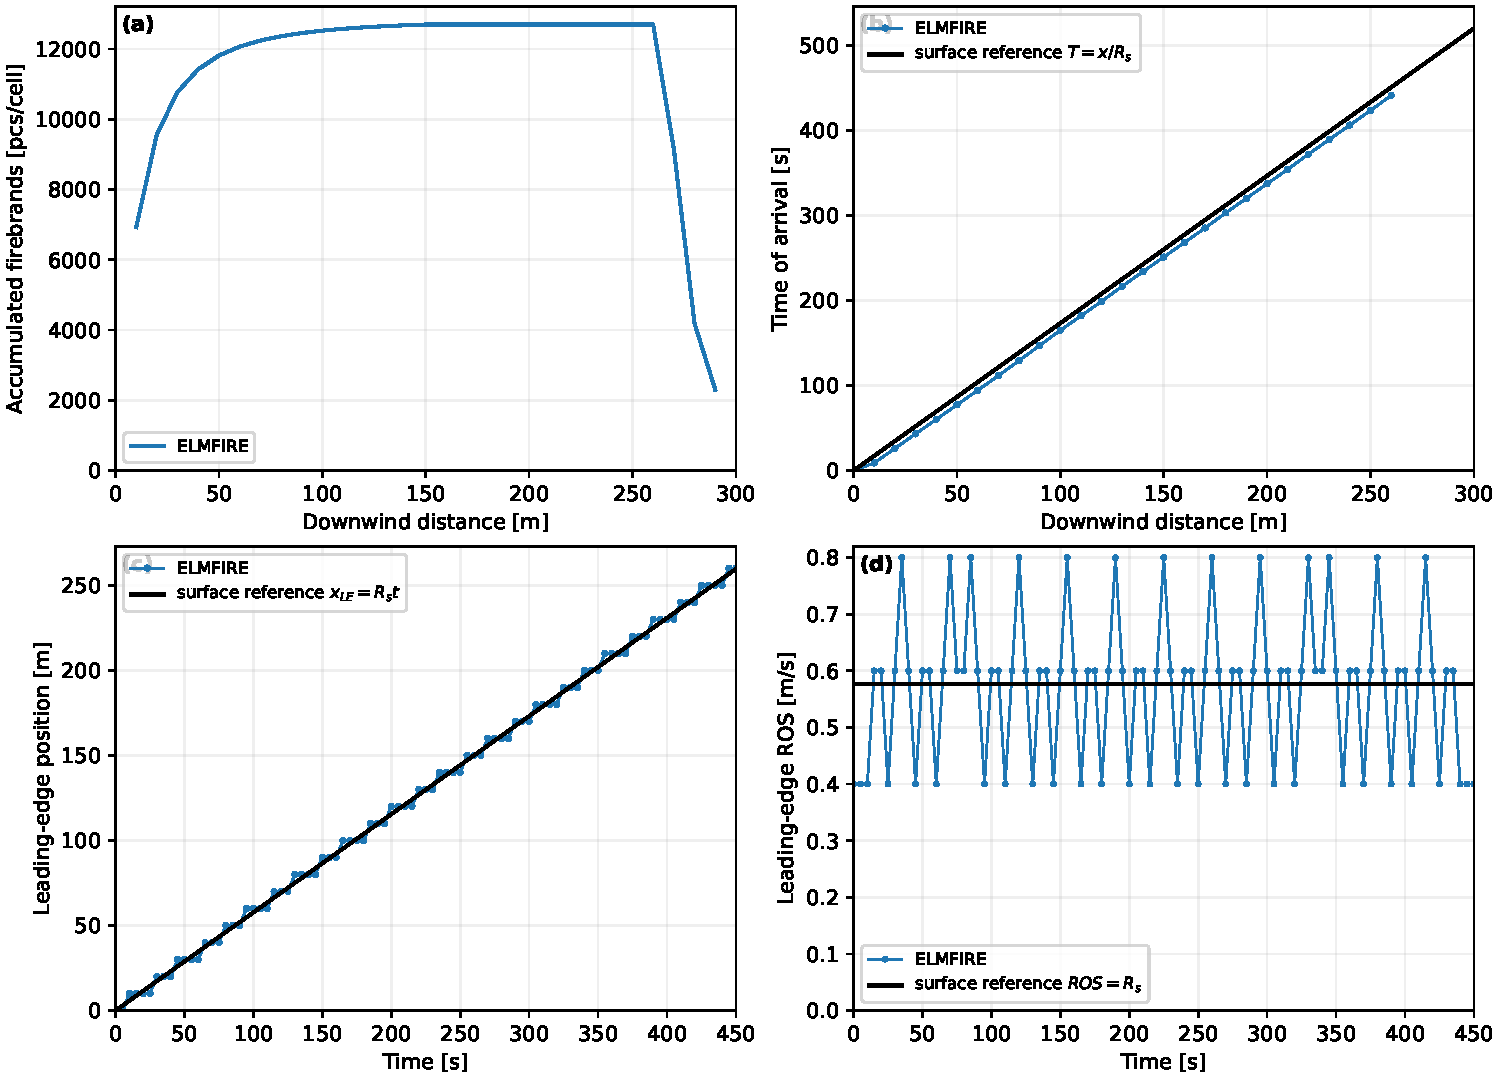
\includegraphics[width=0.96\textwidth,height=0.66\textheight,keepaspectratio]{../figures/surface_dominated_reference.pdf}
\caption{Long-delay surface-dominated variant. The leading edge remains close
to the surface-spread characteristic despite continued firebrand deposition.}
\label{fig:surface-dominated-reference}
\end{figure}

\begin{figure}[H]
\centering
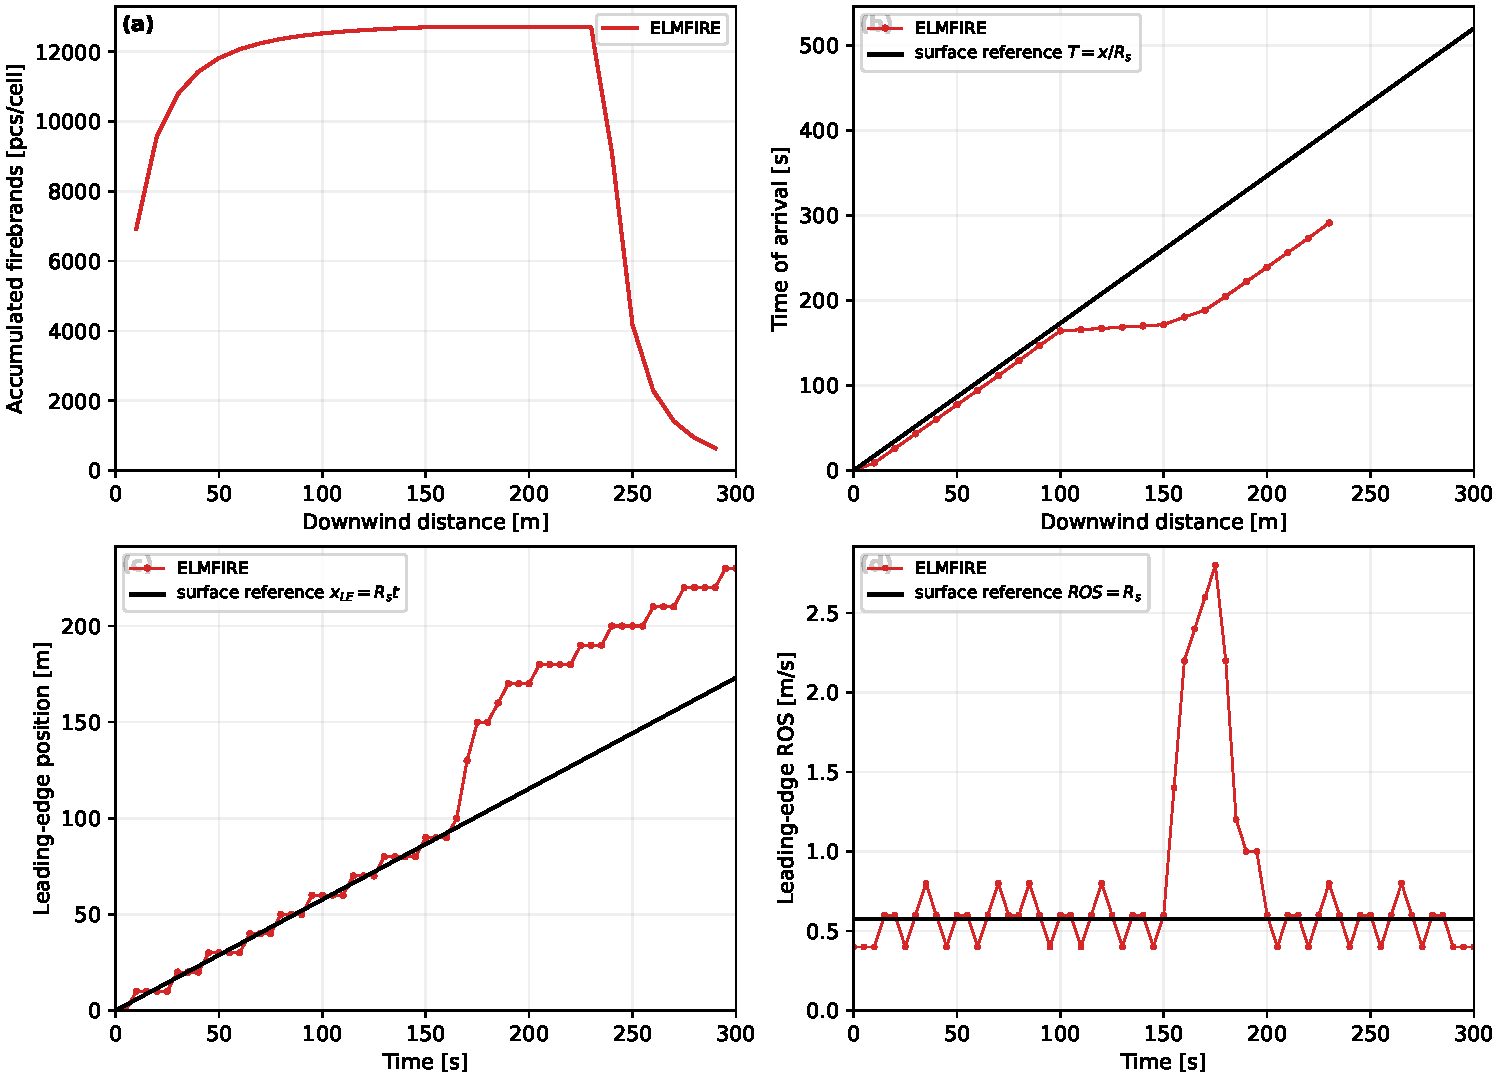
\includegraphics[width=0.96\textwidth,height=0.66\textheight,keepaspectratio]{../figures/mixed_mode_reference.pdf}
\caption{Finite-delay mixed-mode variant. Departure from the surface-only
arrival, trajectory, and ROS references identifies firebrand-induced advance.}
\label{fig:mixed-mode-reference}
\end{figure}

Figure~\ref{fig:delay-effect} overlays the two variants as a supplemental
controlled comparison, making the timing and magnitude of their divergence
easier to identify.

\begin{figure}[H]
\centering
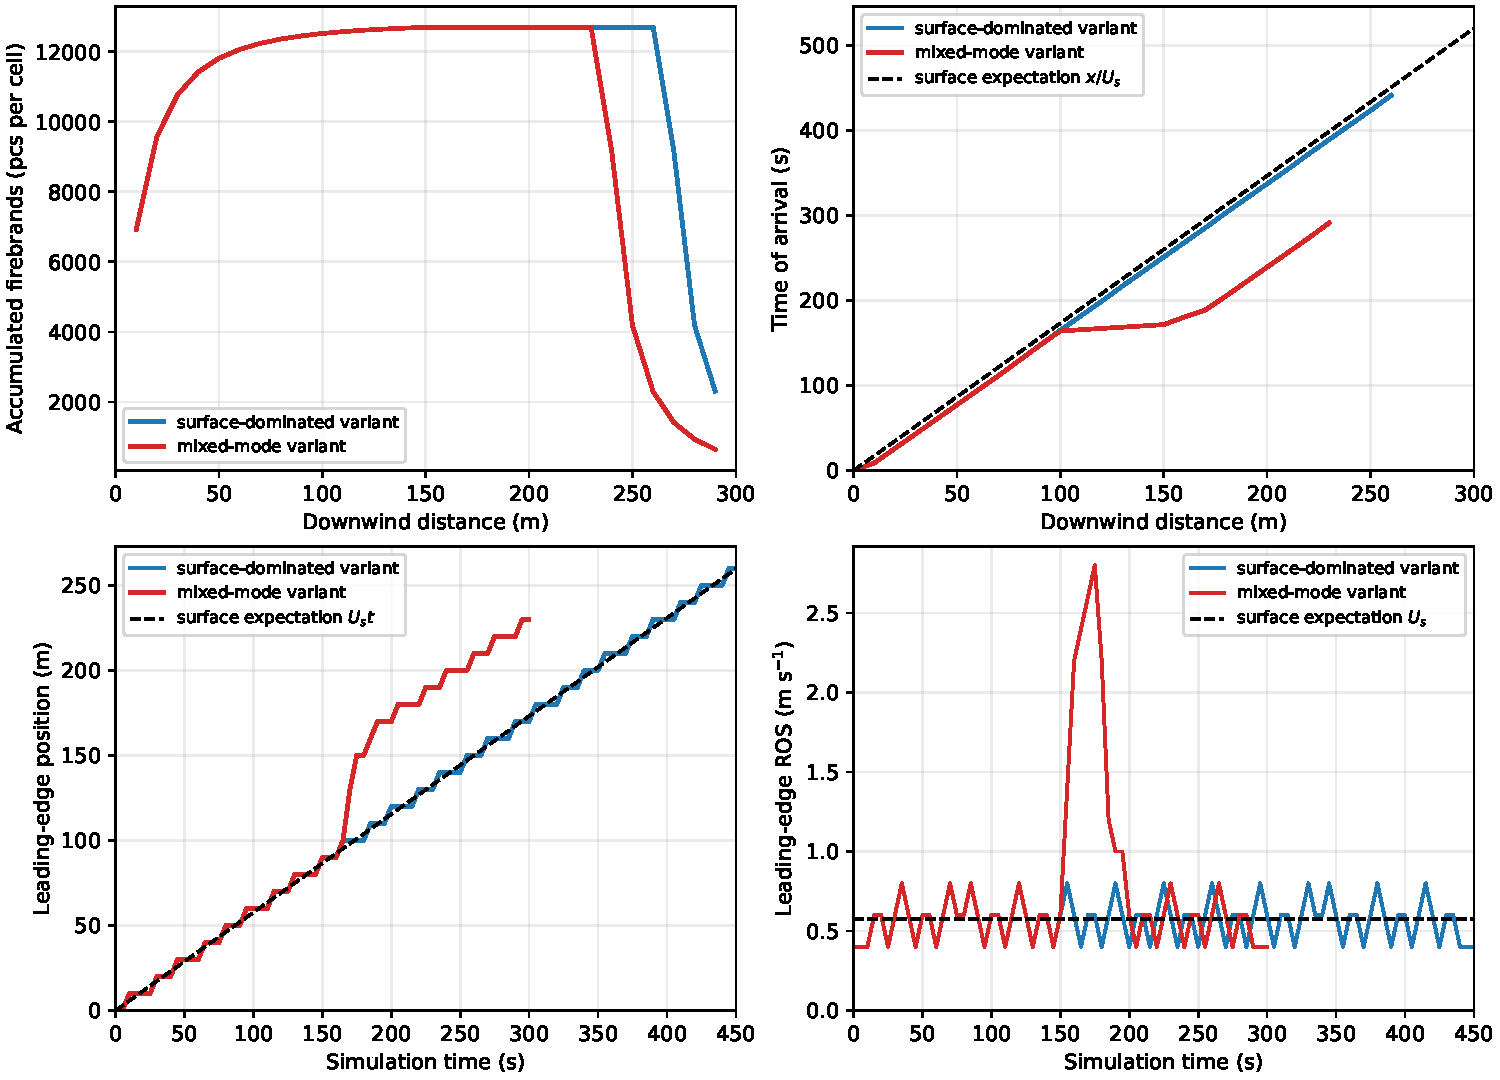
\includegraphics[width=0.96\textwidth,height=0.66\textheight,keepaspectratio]{../figures/mixed_mode_delay_effect.pdf}
\caption{Paired ELMFIRE comparison of the long-delay surface-dominated and
finite-delay mixed-mode regimes. Accumulation is crosswind averaged; the other
panels use the centre-row arrival-time field.}
\label{fig:delay-effect}
\end{figure}
\FloatBarrier

\section{Calculated metrics and verification decision}

Table~\ref{tab:metrics} reads the calculated entries directly from
\path{outputs/metrics.json}. An empty simulation result is represented as
N/A with NOT EVALUABLE, never as an empty table cell or an implicit pass.

\begin{table}[H]
\centering
\small
\caption{Acceptance metrics calculated from the paired ELMFIRE outputs.}
\label{tab:metrics}
\begin{tabular}{llll}
\toprule
Metric & Acceptance limit & Calculated & Status \\
\midrule
Output completeness & 2 variants & \Metric{completedvariants}/2 & \Metric{status} \\
surface-dominated variant mean TOA error & $\le 0.10$ & \Metric{surfacedominatedtoameanrelativeerror} & \Metric{surfacedominatedtoastatus} \\
surface-dominated variant mean ROS (\si{\metre\per\second}) & $\Metric{surfacerosreferencemps}\mathbin{\pm}10\%$ & \Metric{surfacedominatedmeanrosmps} & \Metric{surfacedominatedrosstatus} \\
surface-dominated variant ember-ignited cells & $\le 0$ & \Metric{surfacedominatedemberignitioncells} & \Metric{surfacedominatedignitionstatus} \\
mixed-mode variant ROS / $U_s$ & $\ge 1.10$ & \Metric{mixedmoderosratiotosurface} & \Metric{mixedmoderosstatus} \\
mixed-mode variant ember-ignited cells & $\ge 1$ & \Metric{mixedmodeemberignitioncells} & \Metric{mixedmodeignitionstatus} \\
mixed-mode variant edge gain at 250 s (m) & $\ge 20$ & \Metric{mixedmodeleadingedgegainm} & \Metric{mixedmodeedgegainstatus} \\
mixed-mode variant acceleration onset (s) & $120$--$220$ & \Metric{mixedmodeaccelerationonsets} & \Metric{mixedmodeonsetstatus} \\
Median mixed-mode variant TOA lead (s) & $\ge 20$ & \Metric{pairedmediantoaleads} & \Metric{pairedtoastatus} \\
\midrule
Overall decision & all components pass & \Metric{verificationpassed} & \Metric{status} \\
\bottomrule
\end{tabular}
\end{table}

\section{Technical interpretation}

A pass demonstrates two complementary properties: delayed firebrand states do
not spuriously outrun the surface solver in the surface-dominated limiting
case, and reducing the delay activates a resolvable acceleration in the
mixed-mode variant.
If surface-dominated variant fails alone, inspect the physical mass threshold, development-state
timing, and arrival-time update. If mixed-mode variant fails alone, inspect the simple
ignition probability, persistence of deposited ember states across level-set
steps, delayed transition to a full ignition, and the coupling that writes
that ignition to the level set.

This is code verification of the controlled formulation, not field validation.
The ELMFIRE experiment is two-dimensional but deliberately uses a
uniform crosswind line so the centre transect approximates the corresponding
one-dimensional calculation. The mixed-mode thresholds diagnose the expected
mixed regime rather than an unavailable closed-form mixed-mode solution.
Stochastic ignition means the exact onset may vary, which is why its
acceptance window brackets rather than equals \SI{172.4}{\second}.

To reproduce the result from this directory, export an absolute
\path{ELMFIRE_BIN} and run \path{./run_case.sh}. The current processing note
is: \Metric{notes}

\section{Scope and limitations}
This paired test isolates the interaction between surface propagation and firebrand ignition delay in a uniform domain. It verifies implementation behavior and timing attribution; it does not validate either spread mechanism against field observations.

\begin{thebibliography}{9}
\bibitem{Qin2025}
Y. Qin, \emph{A Physics-Based Eulerian Framework for Modeling Firebrand
Showering in Regional-Scale Wildland and Wildland--Urban Interface Fire
Simulations}, Ph.D. dissertation, University of Maryland, College Park, 2025.
\end{thebibliography}
